\documentclass{article}
\usepackage{xcolor}
\usepackage{tikz}
\usetikzlibrary{scopes}
\usepackage{verbatim}

\begin{document}


%\tikzstyle{block} = [draw, rectangle, minimum width = 0.75cm, minimum height = 0.75cm]


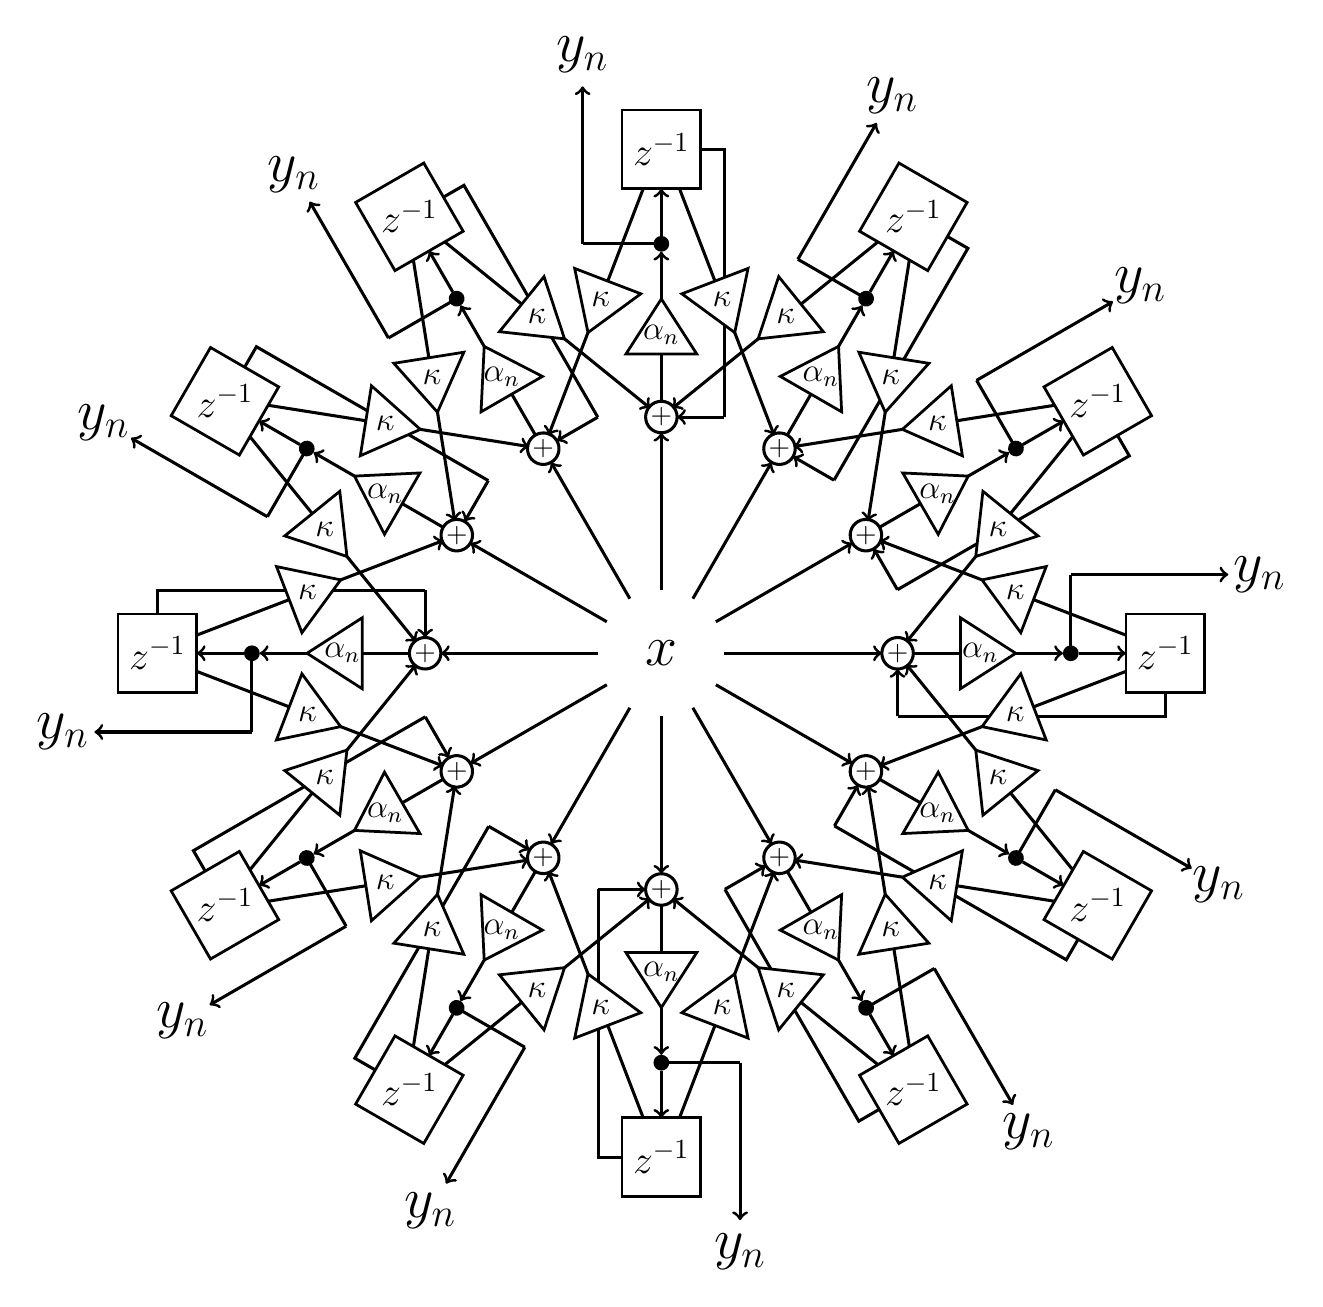
\begin{tikzpicture}[line width=1.1pt]

    \def\unit_delay{
      \filldraw[fill=white,draw=black, line width=1pt,sharp corners] (-0.5,-0.5) -- (-0.5,0.5) -- (0.5,0.5)  -- (0.5,-0.5) -- cycle;
      \draw(0,0) node {\Large$z^{-1}$};
    }

    \def\factor#1{
      \filldraw[fill=white,draw=black, line width=1pt,sharp corners] (-0.2,-0.3) -- (-0.2,0.3) -- (0.3,0) -- cycle;
      \draw(0.2,.45) node {\Large #1};
    }

    \def\factorr#1{
      \filldraw[fill=white,draw=black, line width=1pt,sharp corners] (-0.3,-0.45) -- (-0.3,0.45) -- (0.4,0) -- cycle;
      \draw(-0.05,0) node {\large #1};
    }

    \def\xline#1{
      \draw[->] (0,0) -- (#1,0);
    }

    \def\interlines{
        %\draw[->] (0,0) -- ( -3.5,  0.95 );  % 20
        %\draw[->] (0,0) -- ( -3.5, -0.95 );
        %\draw[->] (0,0) -- ( -3.57,  1.12 );   % 30
        %\draw[->] (0,0) -- ( -3.57, -1.12 );
        \draw[->] (0,0) -- ( -3.7,  1.45 );   % 30
        \draw[->] (0,0) -- ( -3.7, -1.45 );
    }

    \def\coupling{
      \begin{scope}[ rotate = 159 ]
        \begin{scope}[ shift = ({ 0.0 , 0 }) ] \xline{2.0}           \end{scope}
        \begin{scope}[ shift = ({ 2.2 , 0 }) ] \factorr{$\kappa$}   \end{scope}
        \begin{scope}[ shift = ({ 2.6 , 0 }) ] \xline{1.4}            \end{scope}
      \end{scope}
      \begin{scope}[ rotate = -159 ]
        \begin{scope}[ shift = ({ 0.0 , 0 }) ] \xline{2.0}           \end{scope}
        \begin{scope}[ shift = ({ 2.2 , 0 }) ] \factorr{$\kappa$}   \end{scope}
        \begin{scope}[ shift = ({ 2.6 , 0 }) ] \xline{1.4}            \end{scope}
      \end{scope}
    }

    \def\dot#1{
      \fill(0,0) circle(#1);
    }

    \def\adder{
      \draw circle(0.2);
      \node(0,0) {$+$};
    }

    \def\output{
      \draw     (0,0) -- (0,1);
      \draw[->] (0,1) -- (2,1) node[pos=1.2] {\huge $y_n$};
    }

    \def\feedback{
      \draw     (0,0) -- (0,-.8) -- (-3.4,-.8);
      \draw[->] (-3.4,-.8) -- (-3.4,-.2);
    }


    \node(0,0) { \huge $x$ };

    %\foreach \phi in{0,24,...,336}
    \foreach \phi in{0,30,...,330}
    \begin{scope}[ rotate = \phi ]
      \begin{scope}[ shift = ({ 0.8 , 0 }) ] \xline{2.0}           \end{scope}
      \begin{scope}[ shift = ({ 3.0 , 0 }) ] \adder           \end{scope}
      \begin{scope}[ shift = ({ 3.2 , 0 }) ] \xline{0.8}           \end{scope}
      \begin{scope}[ shift = ({ 4.1 , 0 }) ] \factorr{$\alpha_n$}   \end{scope}
      \begin{scope}[ shift = ({ 4.5 , 0 }) ] \xline{.6}            \end{scope}
      \begin{scope}[ shift = ({ 5.2 , 0 }) ] \dot{.1}              \end{scope}
      \begin{scope}[ shift = ({ 6.4 , 0 }) ] \feedback           \end{scope}
      \begin{scope}[ shift = ({ 5.2 , 0 }) ] \output            \end{scope}
      \begin{scope}[ shift = ({ 5.3 , 0 }) ] \xline{.6}            \end{scope}
      \begin{scope}[ shift = ({ 6.5 , 0 }) ] \coupling           \end{scope}
      \begin{scope}[ shift = ({ 6.4 , 0 }) ] \unit_delay           \end{scope}
    \end{scope};


\end{tikzpicture}
\end{document}

